\section{Methods}
	
	\subsection{Preprocessing}\label{sec: proprocessing}
	In order to classify the given data into smaller test sets or mask different aspects, we have to perform some analysis.\\
	We observe that even though we have 124979 individual lines defining a movement, there is one line defining a \texttt{NotANumber}-exception and therefore gets neglected for further usage.	\\
	We provide the \texttt{testDataGenerator} python script. Through flags and input arguments, the script is able to create all test sets used by our clustering and neural net approaches.\\
	We observe the following distribution over the whole dataset:\\
	
	\vspace*{-3em}
	\begin{figure}[H]
		\centering		
		\setlength\tabcolsep{.2cm}
		\begin{tabular}{c|ccccccc}
			strata &  1   &   2   &   3   &  4   &  5   &  6   & $\Sigma$ \\ \hline
			abs   & 6963 & 52265 & 49404 & 8772 & 5536 & 2038 &  124978  \\
			\%   & 5.57 & 41.82 & 39.53 & 7.02 & 4.43 & 1.63 &   100
		\end{tabular}
		\vspace*{-2.5em}
		\label{table: distribution normal}
	\end{figure}
	There is an upper bound on equal distribution through strata 6. It has at most 2038 individual elements.
	Furthermore we have to make sure that two different data points, which belong to the very same person, are assigned to the same cluster. To do so, we compute the value \texttt{ID}, which identifies each person and can be used to combine movements that are considered to be from the same person. I.e. two movements correspond with the very same person, if and only if they are consecutive in the original dataset and have the same strata, age and gender. This approach is taken since the surveys are concatenated sequentially and it is unlikely, that multiple consecutive movements with same strata, age, gender belong to two different persons.\\
	
	\vspace*{-3em}
	\begin{figure}[H]
		\centering
		\setlength\tabcolsep{.2cm}
		\begin{tabular}{c|ccccccc}
			strata &  1   &   2   &   3   &  4   &  5   &  6  & $\Sigma$ \\ \hline
			abs   & 3153 & 23367 & 21418 & 3497 & 2083 & 595 &  54113   \\
			\%   & 5.83 & 43.18 & 39.58 & 6.46 & 3.85 & 1.1 &   100
		\end{tabular}
		\vspace*{-2.5em}
	\end{figure}
	Following, we introduce vectors representing single persons. Since strata 6 is the smallest strata with 595 persons, it limits the size of an equally distributed dataset where each data point coincides with one person.\\
	
	\textbf{Stratified Person Data}\label{subsubsec: person vector data}\\
	As stated before, instead of simple IDs for every person we expand the parsing by using a data encapsulating in a class called \texttt{Person}. This class stores the ID, the parameters defining a person (c.f. \Cref{sec: proprocessing}), and all movements from that person.\\
	Then we are able to compute the following vector, with 850 entries, for further usage, that combines all movements of the person:
	\begin{align*}
	\underbrace{\#o_1, \dots, \#o_{413}, \#d_1, \dots, \#d_{413}}_{2\cdot 413} ,
	\underbrace{\mathit{AM}, \mathit{MD}, \mathit{PM}, \mathit{MN}}_{4}, 
	\underbrace{\#r_1, \dots, \#r_7}_{7}, \\
	\underbrace{\#\mathit{MoT}_1, \dots, \#\mathit{MoT}_7}_{7}, \underbrace{\mathit{S_{Dest}}, \mathit{S_{Dist}}, \mathit{G}, \mathit{A} ,\mathit{strata}, \mathit{strataGrouped}}_{6}
	\end{align*}
	with the following abbreviations ($1 \le i \le 413$, $1 \le j \le 7$):
	\begin{figure}[H]
		\centering
		\hspace*{-.3cm}
		\begin{subfigure}{0.50\textwidth}
		\begin{itemize}
			\setlength{\itemindent}{.4cm}
			\item[$o_i$:]  the $i$-th origin data point
			\item[$d_i$:]  the $i$-th destination data point
			\item[$\mathit{AM}$:] movements at time stamp AM
			\item[$\mathit{MD}$:] movements at time stamp MD
			\item[$\mathit{PM}$:] movements at time stamp PM
			\item[$\mathit{MN}$:] movements at time stamp MN
			\item[$r_j$:] the $j$-th reason
		\end{itemize}
	\end{subfigure}\hspace*{1cm}
	\begin{subfigure}{0.48\textwidth}
	\begin{itemize}
			\item[$\mathit{MoT}_j$:] the $j$-th mean of transportation
			\item[$\mathit{S_{Dest}}$:] sum of all durations
			\item[$\mathit{S_{Dist}}$:] sum of all distances
			\item[$\mathit{G}$:] the gender
			\item[$\mathit{A}$:] the age
			\item[$strata$:] the strata (used for comparison)
			\item[$strataGrouped$:] the aggregated stratas
		\end{itemize}
	\end{subfigure}
	\end{figure}


	
	\subsection{Unsupervised learning}
	\subsubsection{Clustering the data}
	
	is in the field of \textit{Data Mining}, \textit{Cluster Analysis} or \textit{Clustering} a process of grouping data objects from a dataset into multiple groups. The essential criterion, for the quality of the clustering, is \textit{similarity}, such that data objects are similar to other objects in the same cluster and dissimilar to objects from other clusters. 
	
	In the scope of this work, we decided to use the well-known partitioning method k-means. In general, given $n$ data objects, partitioning methods distribute the data objects into $k\in\mathbb{N}$ clusters with $k\le n$, using a distance measure to evaluate the respective similarity. 
%	Those methods form exclusive clusters by ensuring that each cluster contains at least one object.
	Note that the number $k$ of clusters has to be chosen manually a-priori and given to the partitioning process.
	
	\subsubsection{k-means}
	
	is a \textit{centroid based technique}, meaning that each cluster is represented by a data point, which at the same time is the centre of the cluster. A distance measure is then used to assign every remaining data object from the data set to the best fitting cluster. This is done according to its similarity to the centre of this cluster and its dissimilarity to the centres of any other cluster.
	
	The data objects within a dataset are considered to reside in an euclidean space. Thus, the euclidean distance is used to calculate a score for the similarity of two data points. When using k-means, the quality of a cluster $C_i$, $i\in [k]$, can be evaluated by computing the sum of squared distances between all data points $p$ in the object space and the centroids $c_i \in C_i$ of every cluster. This method is known as \textit{within-cluster variation} \cite{data_mining} and defined as follows: 
	\begin{equation}
		E = \sum_{i=1}^{k} \sum_{p \in C_i} dist(p, c_i)^2,
	\end{equation}
	Given $k$, the first step of k-Means is to select $k$ random points as cluster centres. Those do not have to be actual data points.
%	objects in the data set as initial representatives for the cluster centres.
	In order to achieve this, each cluster centroid is redefined as the mean of all objects within that cluster. By considering the updated centroids, every data point is reassigned to the now best fitting cluster. This iterative process will continue until no better clustering can be found or a maximal chosen step size is reached.\\
%	\subsubsection{Clustering with RapidMiner}	


	As a tool we consider RapidMiner, since it has many modules already efficiently implemented and is easy to adapt.

	\vspace*{-2em}
	\begin{figure}[H]
		\centering
		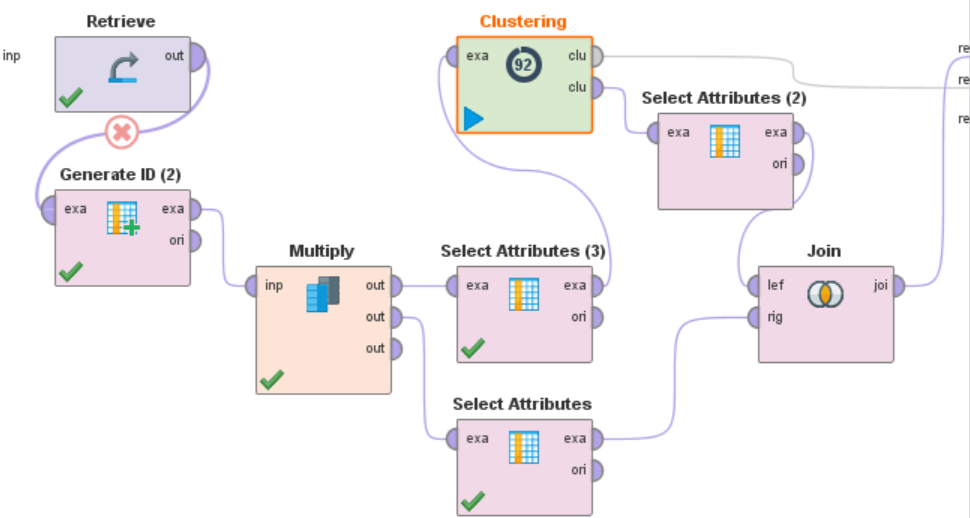
\includegraphics[width=0.9\textwidth]{ClusteringRapid.PNG}
		\caption{Process of k-means clustering}
		\label{fig: kclust}
		%\vspace*{-2em}
	\end{figure}

	The Process (c.f. \Cref{fig: kclust}) contains the following steps:\\

	\begin{tabular}{r c l}
		\textbf{Retrieve} & : &  imports the data into the process \\
		\textbf{Generate ID} & : & creates an ID so we can make the comparison\\
		 & & step at the end through joining the sets\\
		 && based on the ID\\
		\textbf{Multiply} & : & creates two identical data sets\\
		\textbf{Select Attributes} & : &  removes the strata before the clustering step,\\
		& & everything except cluster and ID after the clustering \\
		& & and just keeps ID and strata for the join step\\
		\textbf{Clustering} & : &  runs the k-means clustering algorithm. The number of \\
		& & clusters has to be fixed \\
		\textbf{Join} & : & For comparing the clustering result and the strata, we \\
		& & join the two filtered data sets on the ID \\
	\end{tabular}
	
	In the clustering block, we can choose between different distance measures and maximal step numbers. We keep the default configuration and choose the mixed euclidean distance measure.
%	We decide to concentrate on almost everywhere basic configurations and chose the squared euclidean distance in the mixed version.
\vspace*{-1em}
	\subsubsection{Gower distance{\normalfont,}}\label{gower} in contrast to the popular distance measures, can also handle the mixed data within the given dataset. The Gower distance measure distinguishes between three types of variables: binary, categorical and numerical.
%	When clustering data with algorithms such as \textit{k-means}, the distance between data points is usually calculated by measures such as the Euclidean or Manhattan norm.
%	These distance measures come with constraints though, since they are only defined for numerical variables. 
	%In the scope of this work, we are facing data points with mixed variable types.
	%, therefore we investigated the \textbf{Gower distance measure} as an appropriate measure to calculate an overall \textit{similarity} between mixed data points. 
%	\\ \textbf{Binary} variables, where two variables of value 0 are \textit{not} considered as match \cite{gower1971general}. In the scope of this work, the only considerable candidate for a binary variable would have been \textit{gender}. Though, during our research process, we concluded that the similarity measure for binary variables was not a suitable choice, as the distance does not match 0 values. Hence, we consider all variables, that are not explicitly numerical, as categorical variables.\\
%	\textbf{Categorical} variables form a set of unordered values and are comparable to ENUMs in programming languages.\\	
%	\textbf{Numerical} variables hold ordered numerical values that support arithmetic operations.
%	\subsubsection{Calculating the distances}
	The distance can be calculated as follows:
	
	Given two data points $x$ and $y$, each form a tuple of $v$ variables of arbitrary type, the similarity coefficient is given by:
	\begin{equation}\label{eq1}
	S_{xy} = \sum_{k=1}^{v} s_{xy,k} / \sum_{k=1}^{v} \delta_{xy,k} 
	\end{equation} 
	where $s_{xy,k}$ denotes a \textit{score for the similarity} of the two variables at the $k$-th entry in the data points $x$ and $y$. Note, that the definition of the score depends on the
	%Timo nervt
	type of the variable, as defined below. In the divisor, $\delta_{xy,k}$ basically represents the possibility of comparing the two variables at index $k$, such that it evaluates to 1, if the two variables are comparable and to 0 if not. %PASS AUF
	For example, variables are not comparable, if values are undefined in the data points or the variable types do not match. Within this work, the dataset is complete, therefore, $\sum_{k=1}^{v} \delta_{xy,k}=v$. Thus, the similarity coefficient in equation \hyperref[eq1]{(2)} can be interpreted as the average value of all similarity scores. 
	With respect to the variable type, the similarity score $s_{xy,k}$ is defined as follows:\\
	\\ \textbf{Binary:} The score for binary variables is basically the result of an logical conjunction operation. As pointed out above, 0 values are considered to be not a match, thus not even considered to be comparable. Hence, the values result as in the table
		\begin{center}
			\begin{tabular}{l | c c c r}
				i & 1 & 1 & 0 & 0 \\
				j & 1 & 0 & 1 & 0 \\
				\hline
				$s_{xy,k}$ & 1 & 0 & 0 & 0 \\
				$\delta_{xy,k}$ & 1 & 1 & 1 & 0
			\end{tabular}
		\end{center}	
	\textbf{Categorical:} The similarity score of categorical variables is 1, if the variables are completely identical in $x$ and $y$, and 0, if they differ.
	
	\textbf{Numerical:} For numerical variables, the similarity score is calculated by
		\begin{equation*}
		s_{xy,k} = 1 - \frac{\vert x_k - y_k \vert}{range(k)}
		\end{equation*}
		where $range(k)$ is the total range of values, that the numerical attribute at index $k$ can accept. This can be a global maximum of acceptable values for attribute $k$, or chosen on the basis of the dataset.

\subsubsection{Principal component analysis}

(PCA) uses an orthogonal transformation to convert a dataset, with correlated data, into a dataset without correlations and decreased dimension. This is a helpful technique to get a better understanding of the data complexity, as well as decreasing the time consumption in further steps.

The first component for the PCA transformation, the weight matrix, has to satisfy the following:

\vspace*{-1em}
\begin{align*}
w_1 &= \text{argmax}_{\|w\| = 1} \{\sum_i (t_1)_i^2\}\\
	&= \text{argmax}_{\|w\| = 1} \{\sum_i (x_iw)^2\}
	\vspace*{-2em}
\end{align*}


which is achieved by the corresponding eigenvector.

The next components need to fullfill:
\begin{align*}
\hat{X}_k &= X - \sum_{s=1}^{k-1} Xw_sw_s^T\\
w_k &= \text{argmax}_{\|w\| = 1} \{\|\hat{X}_kw\|^2\}\\
	&= \text{argmax}_{\|w\| = 1} \{\frac{w^T\hat{X}_k^T\hat{X}_kw}{w^Tw}\}
	\vspace*{-1em}
\end{align*}

Based on the weight matrix a mapping is possible from the original space to a new space in which the dataset is uncorrelated. 
	
	\vspace*{-1em}
	\begin{figure}[H]
	\centering
	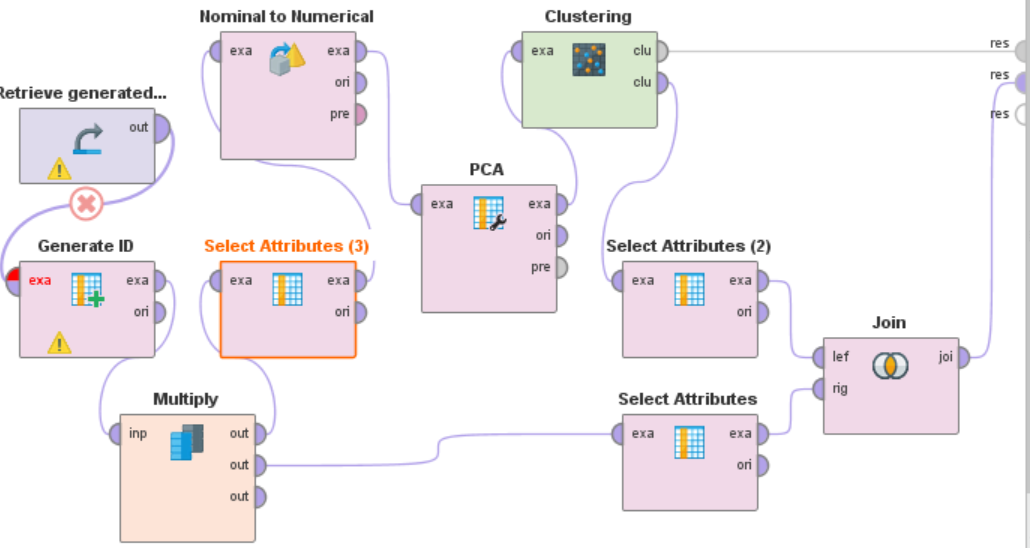
\includegraphics[width=0.9\textwidth]{PCAClustering}
	\caption{RapidMiner process for PCA and k-means}
	\label{fig:PCA}
	\vspace*{-2em}
	\end{figure}

The Process does the following steps, visible in \Cref{fig:PCA}:

\begin{tabular}{r c l}
	\textbf{Retrieve} & : & imports the data in the process.\\
	\textbf{Generate ID} & : & creates an idea for the join later\\
	\textbf{Select Attribute} & : & gives the chosen attributes back\\
	\textbf{Nominal to Numerical} & : & changes the nominal data to numerical data, so \\
	&&that we can apply PCA in the next step \\
	\textbf{PCA} & : & applies the PCA reduction to the data\\
	&& threshold $0.95$ \\
	\textbf{Clustering} & : &  clusters the given data \\
	\textbf{Join} & : & joins the clustering outcome and the strata by the\\
	&& ID\\
\end{tabular}	
		
		
	\subsection{Supervised learning}
	
	\subsubsection{Decision Trees} are a good manner to figure out, which parts of the data set have the most influence on the decision. Therefore, labelled data is needed, which we have given with the strata. We again used RapidMiner for building trees, based on different data sets. 

	\vspace*{-2em}
	\begin{figure}[H]
		\centering
		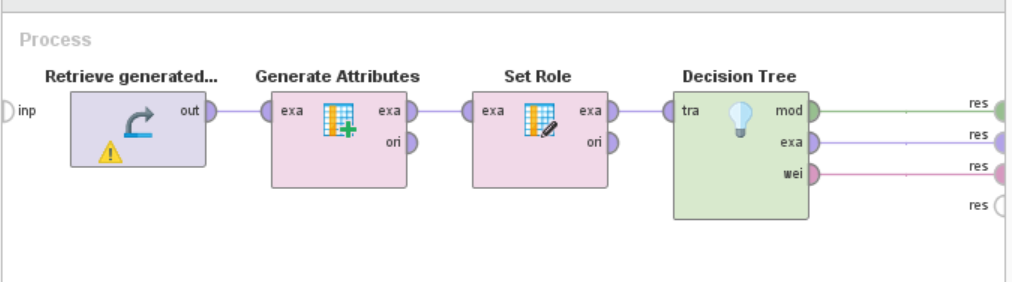
\includegraphics[width = 0.9\textwidth]{DecisionTreeRapidModel.PNG}
		\caption{Process for decision trees in RapidMiner}
		\label{fig: RapDec}
		\vspace*{-1.5em}
	\end{figure}
	
	RapidMiner does the following steps, illustrated in \Cref{fig: RapDec}:
	
	\begin{tabular}{r c l}
		\textbf{Retrieve} & : & includes the dataset\\
		\textbf{Select Attributes} & : & makes it possible to have a look at grouped\\
		&& strata or normal strata\\
		\textbf{Set Role} & : & gives strata the label role, so that the decision tree\\
		&& has those as leafs\\
		\textbf{Multiply} & : & clones the data set \\
		\textbf{Decision Tree} &: & creates the decision tree\\
		\textbf{Apply Model} & : & creates the labelled data set for the \textbf{Performance} step\\
		\textbf{Performance} & : & gives the performance result of the created model\\
	\end{tabular}
	
	We tried several configurations regarding the splitting criterion and  confidence threshold, but the results were similar.
	\vspace*{-1em}

	\subsubsection{Neural Net}
	% TODO
	% like k-means
	are based on biology. In detail, based on the neurons and synapses within the human brain. There a neuron fires to any further connected neurons, if a weighted sum minus a bias value is above a certain threshold.
%	The individual weights and biases are learned by the net.
	Through iteration-wise computing the result and comparing it to the expected outcome, called label, and the use of various machine learning techniques the net is able to adjust the weights and biases \cite{neuralNet}.
	
	\vspace*{-2em}
	\begin{figure}[H]
		\centering
		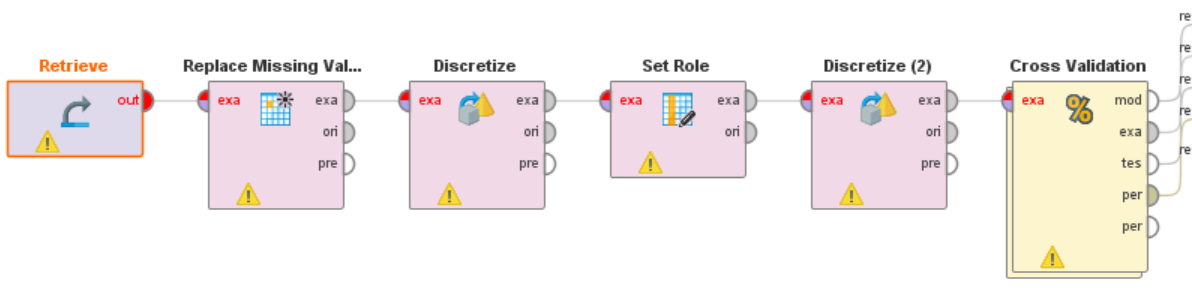
\includegraphics[width = 0.9\textwidth]{RapidNN.PNG}
		\caption{RapidMiner process for neural nets}
		\vspace*{-1em}
	\end{figure}
	
	\begin{tabular}{r c l}
		\textbf{Retrieve} & : & includes the dataset\\
		\textbf{Replace Missing Values} & : & ensure applicable data\\
		\textbf{Discretize} & : & translates numerical to nominal data \\
		\textbf{Set Role} & : & gives strata the label role, so that the decision tree\\
		&& has those as leafs\\		
		\textbf{Cross Validation} & : & models the neural network \\
	\end{tabular}
	